\chapter{Boolean Algebra \& Logic Gates}

Boolean algebra is a branch of mathematics that deals with logical operations on binary variables.

\section{Boolean Operations}

\subsection{Logical Operations}

Logical operations treat any non-zero argument as true.

\subsection{Bitwise Operations}

\subsection{Shift Operations}

\section{Rules and Theorems}

Associative, demorgan, blah blah

\section{Basic Logic Gates}

Put these in a 3x2 table with all three side by side

\subsection{AND}

\begin{figure}[h!]
	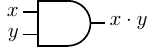
\includegraphics{./img/and.png}
\end{figure}

\begin{tabular}{c c c}
	\hline
	\textbf{x} & \textbf{y} & \textbf{x \& y} \\ 
	\hline
	0 & 0 & 0 \\
	0 & 1 & 0 \\
	1 & 0 & 0 \\
	1 & 1 & 1 \\
	\hline 
\end{tabular} \\

\subsection{OR}

\begin{figure}[h!]
	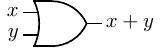
\includegraphics{./img/or.png}
\end{figure}


\begin{tabular}{c c c}
	\hline
	\textbf{x} & \textbf{y} & \textbf{x + y} \\ 
	\hline
	0 & 0 & 0 \\
	0 & 1 & 1 \\
	1 & 0 & 1 \\
	1 & 1 & 1 \\
	\hline 
\end{tabular} \\

\subsection{NOT}

\begin{figure}[h!]
	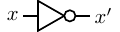
\includegraphics{./img/not.png}
\end{figure}


\begin{tabular}{c c}
	\hline
	\textbf{x} & \textbf{¬x} \\ 
	\hline
	0 & 1  \\
	1 & 0  \\
	\hline 
\end{tabular} \\

\section{Expressions and Simplifications}

Sum of products, product of sums, rules

\section{Karnaugh Maps (K-Maps)}

\section{Latches}

A latch is a circuit that stores one bit of output data directly based on input values.

\subsection{S-R Latch}

\begin{figure}[h!]
	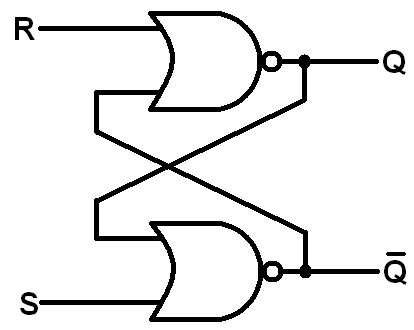
\includegraphics[scale=0.35]{./img/sr-latch.png}
\end{figure}

An S-R latch has two inputs, S and R (Set and Reset). The S input sets the output to 1, and the R input resets the output to 0. An SR latch's output behavior is undefined when both the S and R inputs are at 1. \\

\begin{tabular}{c c c c}
	\hline
	\textbf{S} & \textbf{R} & \textbf{Q} & \textbf{¬Q} \\ 
	\hline
	0 & 0 & Latch & Latch\\
	0 & 1 & 0 & 1\\
	1 & 0 & 1 & 0 \\
	1 & 1 & 0 & 0 \\
	\hline 
\end{tabular} \\

\subsection{Gated SR Latch}

\subsection{D Latch}

\section{Flip-Flops}

\section{S-R Flip-Flop}

\section{References}

\begin{itemize}
	\item https://bob.cs.sonoma.edu/IntroCompOrg-x64/bookch4.html
	\item https://www.allaboutcircuits.com/textbook/digital/chpt-10/s-r-latch/
\end{itemize}